\documentclass{report}
\usepackage[utf8]{inputenc}
\usepackage[english, russian]{babel}
\usepackage{listings}
\usepackage{graphicx}
\usepackage{float}
\graphicspath{{imgs/}}
\usepackage{amsmath,amsfonts,amssymb,amsthm,mathtools} 
\usepackage{pgfplots}
\usepackage{filecontents}
\usepackage{indentfirst}
\usepackage{eucal}
\usepackage{enumitem}
\frenchspacing

\usepackage{indentfirst} % Красная строка

\usetikzlibrary{datavisualization}
\usetikzlibrary{datavisualization.formats.functions}

\usepackage{amsmath}

\definecolor{bluekeywords}{rgb}{0,0,1}
\definecolor{greencomments}{rgb}{0,0.5,0}
\definecolor{redstrings}{rgb}{0.64,0.08,0.08}
\definecolor{xmlcomments}{rgb}{0.5,0.5,0.5}
\definecolor{types}{rgb}{0.17,0.57,0.68}

\usepackage{listings}
\lstset{language=[Sharp]C,
	captionpos=t,
	numbers=left, %Nummerierung
	numberstyle=\small, % kleine Zeilennummern
	frame=single, % Oberhalb und unterhalb des Listings ist eine Linie
	stepnumber=1,                   
	numbersep=5pt,                
	showspaces=false,
	tabsize=2,
	showtabs=false,
	breaklines=true,
	showstringspaces=false,
	breakatwhitespace=true,
	escapeinside={(*@}{@*)},
	commentstyle=\color{greencomments},
	morekeywords={partial, var, value, get, set},
	keywordstyle=\color{bluekeywords},
	stringstyle=\color{redstrings},
	basicstyle=\ttfamily\small,
}


\usepackage[left=2cm,right=2cm, top=2cm,bottom=2cm,bindingoffset=0cm]{geometry}
% Для измененных титулов глав:
\usepackage{titlesec, blindtext, color} % подключаем нужные пакеты
\definecolor{gray75}{gray}{0.75} % определяем цвет
\newcommand{\hsp}{\hspace{20pt}} % длина линии в 20pt
\newcommand{\jj}{\righthyphenmin=20 \justifying}
% titleformat определяет стиль
\titleformat{\chapter}[hang]{\Huge\bfseries}{\thechapter\hsp\textcolor{gray75}{|}\hsp}{0pt}{\Huge\bfseries}


% plot
\usepackage{pgfplots}
\usepackage{filecontents}
\usetikzlibrary{datavisualization}
\usetikzlibrary{datavisualization.formats.functions}
 
\begin{document}
  %\def\chaptername{} % убирает "Глава"
\thispagestyle{empty}
\begin{titlepage}
	\noindent \begin{minipage}{0.15\textwidth}
	
\includegraphics[width=\linewidth]{b_logo.jpg}
	\end{minipage}
	\noindent\begin{minipage}{0.9\textwidth}\centering
		\textbf{Министерство науки и высшего образования Российской Федерации}\\
		\textbf{Федеральное государственное бюджетное образовательное учреждение высшего образования}\\
		\textbf{~~~«Московский государственный технический университет имени Н.Э.~Баумана}\\
		\textbf{(национальный исследовательский университет)»}\\
		\textbf{(МГТУ им. Н.Э.~Баумана)}
	\end{minipage}
	
	\noindent\rule{18cm}{3pt}
	\newline\newline
	\noindent ФАКУЛЬТЕТ $\underline{\text{«Информатика и системы управления»}}$ \newline\newline
	\noindent КАФЕДРА $\underline{\text{«Программное обеспечение ЭВМ и информационные технологии»}}$\newline\newline\newline\newline\newline\newline\newline\newline\newline\newline\newline
	
	
	\begin{center}
		\noindent\begin{minipage}{1.3\textwidth}\centering
			\Large\textbf{  Отчет по лабораторной работе №1}\newline
			\textbf{по дисциплине "Анализ алгоритмов"}\newline\newline
		\end{minipage}
	\end{center}
	
	\noindent\textbf{Тема} $\underline{\text{Расстояние Левенштейна и Дамерау-Левенштейна}}$\newline\newline
	\noindent\textbf{Студент} $\underline{\text{Малышев И. А.}}$\newline\newline
	\noindent\textbf{Группа} $\underline{\text{ИУ7-51Б}}$\newline\newline
	\noindent\textbf{Оценка (баллы)} $\underline{\text{~~~~~~~~~~~~~~~~~~~~~~~~~~~}}$\newline\newline
	\noindent\textbf{Преподаватель: } $\underline{\text{Волкова Л. Л.}}$\newline\newline\newline
	
	\begin{center}
		\vfill
		Москва~---~\the\year
		~г.
	\end{center}
\end{titlepage}


\tableofcontents
  
\newpage
\chapter*{Введение}

\addcontentsline{toc}{chapter}{Введение}

Динамическое программирование - это форма вычислений, при которой следующий член вычисляется на основе предыдущего. Простейшим примером применения является вычисление чисел Фибоначчи. Кроме того, динамическое программирование может применяться и в более сложных задачах таких, как проебразование строк из одной в другую. В этом случае задача сводится к вычислению расстояния Левенштейна (редакционного расстояния) - минимального количества операций вставки, удаления символа или замены символа один на другой, необходимых для преобразования одной строки в другую. Расстояние Левенштейна применяется в следующих областях:
\begin{itemize}
\item компьютерной лингвистике для устранения  ошибок в набираемом тексте;
\item в бионформатике для сравнения генов.
\end{itemize}

Поэтому \textbf{целью} данной работы является получение навыка динамического программирования на примере реализации алгоритмов редакционного расстояния. 

Для достижения поставленной цели необходимо решить следующие \textbf{задачи}:
\begin{enumerate}
\item Изучить алгоритмы расчета редакционного расстояния;
\item Реализовать алгоритмы подсчета редакционного расстояния;
\item Протестировать реализованные алгоритмы;
\item Провести сравнительный анализ реализаций алгоритмов по затраченному процессорному времени и памяти.
\end{enumerate}


\chapter{Аналитическая часть}
В данном разделе определяются расстояния Левенштейна и Дамерау-Левенштейна, а также рассматриваются различные алгоритмы и их модификации для вычисления указанных расстояний.

\section{Расстояние Левенштейна}

Для вычисления редакционного расстояния вводятся следующие цены операций:
\begin{itemize}
\item замена одного символа на другой - 1;
\item вставка символа - 1;
\item удаление символа - 1;
\item совпадение - 0.
\end{itemize}

С учётом этого вводится рекурсивная формула для вычисления расстояния Левенштейна:
\begin{equation}
\label{eq:LD}
D(s1[1..i], s2[1..j]) = 
\begin{cases}
0, &\text{i = 0, j = 0}\\
i, &\text{i > 0, j = 0}\\
j, &\text{i = 0, j >  0}\\
\min \lbrace \\
\qquad D(s1[1..i], s2[1..j-1]) + 1\\
\qquad D(s1[1..i-1], s2[1..j]) + 1 &\text{i > 0, j > 0}\\
\qquad D(s1[1..i-1], s2[1..j-1]) + 
\begin{cases} 
0, &\text{s1[i] = s2[j]}\\
1, &\text{иначе}\\ 
\end{cases}\\
\rbrace
\end{cases}
\end{equation}

\subsection{Рекусивный алгоритм нахождения расстояния Левенштейна}\label{rd}
Данный алгоритм использует для решения формулу \ref{eq:LD}, однако в отличие от прерыдущих является рекурсивным, а значит, для хранения промежуточных результатов используется стек. Кроме того, при этом подходе возникает проблема повторных вычислений, так как функция $D(s1[1..i], s2[1..j])$ будет выполняться несколько раз в разных ветвях дерева вызовов.

\subsection{Нерекусивный алгоритм нахождения расстояния Левенштейна с кэшем в виде матрицы}
Данный алгоритм использует для решения задачи матрицу размером $(m + 1) * (n + 1)$, где $m$ и $n$ - длины двух строк, одну из которых необходимо преобразовать к другой. На каждом шаге работы алгоритма заполняется одна клетка матрицы в соответствии с формулой \ref{eq:LD}. По окончании алгоритма результат будет находиться в последней заполненной клетке.

\subsection{Нерекусивный алгоритм нахождения расстояния Левенштейна с кэшем в виде 2 строк матрицы}
Данный алгоритм является модификацией предыдущего. Очеивдно, что на кажом шаге алгоритма используются значения из текущей и предыдущей строки матрицы, поэтому достаточно хранить только их, а не всю матрицу.

\section{Расстояние Дамерау-Левенштейна}

Дамерау дополнил определение расстояния Левенштейна еще одной операцией, а именно операцией перестановки двух букв местами, стоимость которой тоже равна 1. Расстояние Дамерау-Левенштейна вычисляется по следующей формуле:

\begin{equation}
\label{eq:DLD}
D(s1[1..i], s2[1..j]) = 
\begin{cases}
0,  &\text{i = 0, j = 0}\\
i,  &\text{i > 0, j = 0}\\
j,  &\text{i = 0, j >  0}\\
\min \lbrace \\
\qquad D(s1[1..i], s2[1..j-1]) + 1\\
\qquad D(s1[1..i-1], s2[1..j]) + 1 &\text{i > 0, j > 0}\\
\qquad D(s1[1..i-1], s2[1..j-1]) + 
\begin{cases} 
0, &\text{s1[i] = s2[j]}\\
1, &\text{иначе}\\ 
\end{cases}\\
\left[\begin{array}{ll}
D(s1[1..i-2], s2[1..j-2]) + 1, &\text{если i>1, j>1, s1[i] = s2[j-1], s1[i-1] = s2[j]} \\
\inf, &\text{иначе} \\
\end{array}\right. \\
\rbrace \\
\end{cases} \\
\end{equation}

\subsection{Рекусивный алгоритм нахождения расстояния Дамерау-Левенштейна}

Данный алгоритм использует для решения формулу \ref{eq:DLD} и является рекурсивным, а значит, для хранения промежуточных результатов используется стек. Кроме того, при этом подходе возникает проблема повторных вычислений, так как функция $D(s1[1..i], s2[1..j])$ будет выполняться несколько раз в разных ветвях дерева.

\subsection{Нерекусивный алгоритм нахождения расстояния Левенштейна с кэшем в виде матрицы}

Данный алгоритм решает проблему повторных вычислений простого рекурсивного алгоритма. При данном подходе вводится матрица размером $(m + 1) * (n + 1)$, содержащая уже вычисленные промежуточные результаты. На каждом шаге работы алгоритма заполняется одна клетка матрицы в соответствии с формулой \ref{eq:DLD}. По окончании алгоритма результат будет находиться в последней заполненной клетке.


\section{Вывод}

В данном разделе были даны определения расстояний Левенштейна и Дамерау-Левенштейна, а также рассмотрены 5 алгоритмов вычисления указанных расстояний.
	
\clearpage

\chapter{Конструкторская часть}
В данном разделе разрабатываются схемы алгоритмов на основе их описания, приведённого в аналитическом разделе.
\section{Схемы алгоритмов}\label{schemes}

На рисунках \ref{fig:mpr1}, \ref{fig:mpr2}, \ref{fig:mpr3}, \ref{fig:mpr4} и \ref{fig:mpr5} показаны схемы алгоритма рекурсивного Левенштейна, нерекурсивного алгоритма Левенштейна с кэшем в виде матрицы и двух строк матрицы, рекурсивного алгоритма Дамерау-Левенштейна и нерекурсивного алгоритма с кэшем в виде матрицы соответственно.
\begin{figure}[h!p]\label{recLev}
	\centering
	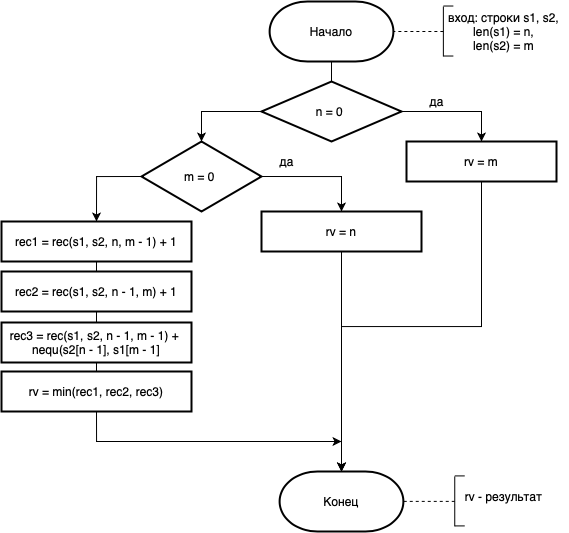
\includegraphics[scale = 0.7]{recLev.drawio.png}
	\caption{Схема рекурсивного алгоритма нахождения расстояния Левенштейна}
	\label{fig:mpr1}
\end{figure}

\begin{figure}[h!p]\label{LevMatr}
	\centering
	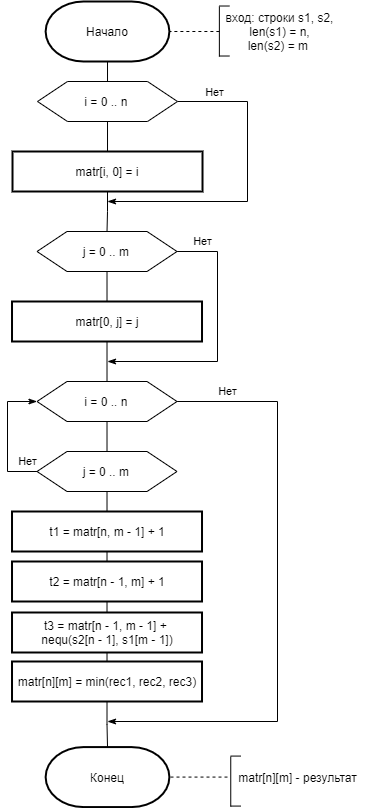
\includegraphics[scale = 0.7]{LevMatr.drawio.png}
	\caption{Схема рекурсивного алгоритма нахождения расстояния Левенштейна с кэшем в виде матрицы}
	\label{fig:mpr2}
\end{figure}

\begin{figure}[h!p]\label{levTwoRows}
	\centering
	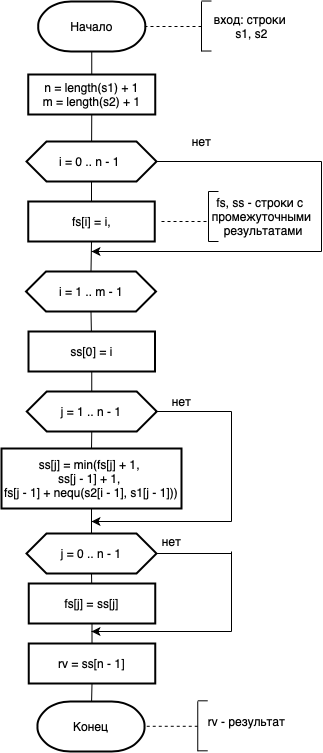
\includegraphics[scale = 0.7]{levRows.drawio.png}
	\caption{Схема нерекурсивного алгоритма нахождения расстояния Левенштейна с кэшем в виде двух строк матрицы}
	\label{fig:mpr3}
\end{figure}

\begin{figure}[h!p]\label{recDam}
	\centering
	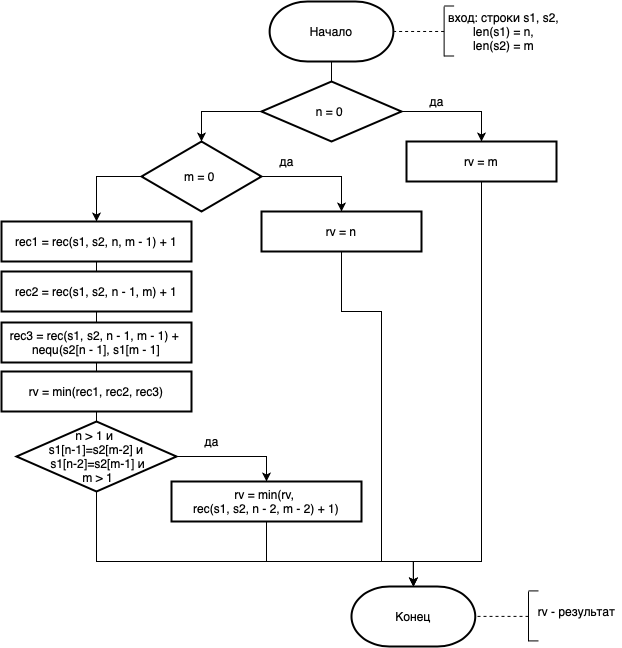
\includegraphics[scale = 0.7]{recDamLev.drawio.png}
	\caption{Схема рекурсивного алгоритма нахождения расстояния Дамерау-Левенштейна}
	\label{fig:mpr4}
\end{figure}

\begin{figure}[h!p]\label{DamMatr}
	\centering
	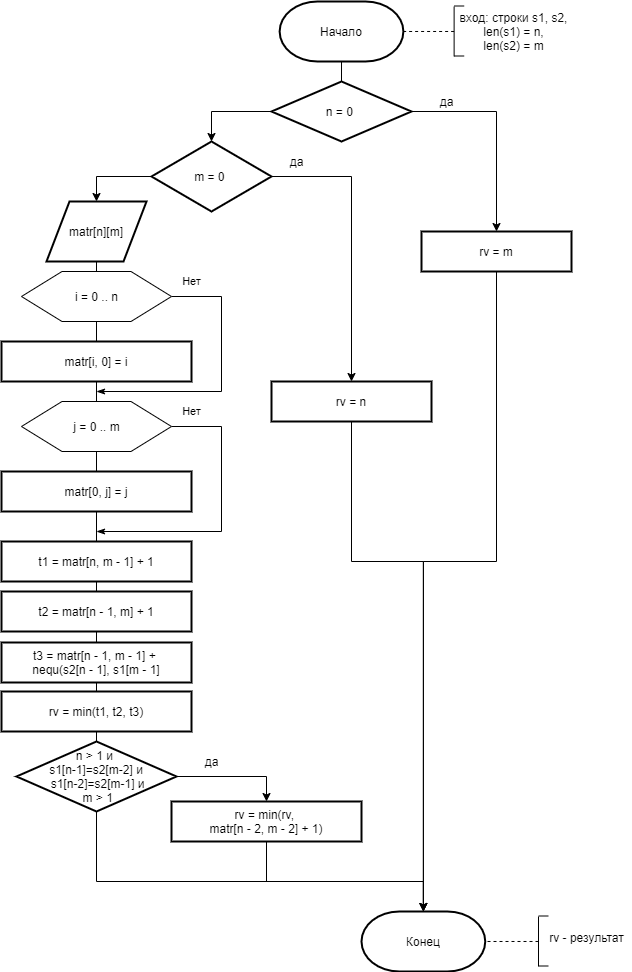
\includegraphics[scale = 0.7]{DamLev.drawio.png}
	\caption{Схема нерекурсивного алгоритма нахождения расстояния Дамерау-Левенштейна с кэшем в виде матрицы}
	\label{fig:mpr5}
\end{figure}

\section{Вывод}

В данном разделе были построены схемы пяти алгоритмов нахождения редакционного расстояния на основе их описания, приведённого в аналитической части.

\newpage

\chapter{Технологическая часть}
В данном разделе приводится реализация алгоритмов, схемы которых были разработаны в конструкторской части. Кроме того, обосновывается выбор технологического стека и проводится тестирование реализованных алгоритмов.
\section{Средства реализации}

В качестве языка программирования был выбран C\#, а среду разработки -- Visual Studio, т. к. я знаком с данным языком и имею представление о тестировании программ в данном языке. Время работы алгоритмов было замерено с помощью библиотеки System.Diagnostics, класса Stopwatch, который имеет методы для расчёта процессорного времени [1].

\section{Реализация алгоритмов}

В листингах 3.1 - 3.5 приведена реализации алгоритмов, описанных в \ref{schemes}.

\begin{lstlisting}[label=code1,caption=Функция для рекурсивного нахождения расстояния Левенштейна]
static int _LevDist(string source, int srclen, string target, int trglen)
{
	if (srclen * trglen == 0)
		return Math.Max(srclen, trglen);
	
	int substitutionCost = 0;
	if (source[srclen - 1] != target[trglen - 1])
		substitutionCost = 1;
	
	int deletion = _LevDist(source, srclen - 1, target, trglen) + 1;
	int insertion = _LevDist(source, srclen, target, trglen - 1) + 1;
	int substitution = _LevDist(source, srclen - 1, target, trglen - 1) + substitutionCost;
	
	return Minimum(deletion, insertion, substitution);
}

static int LevDistRec(string source, string target) =>
	_LevDist(source, source.Length, target, target.Length);
\end{lstlisting}
\newpage
\begin{lstlisting}[label=code2,caption=Функция для нерекурсивного нахождения расстояния Левенштейна с кэшем в виде матрицы]
static int LevDistMatr(string source, string target)
{
	if (source.Length * target.Length == 0)
		return Math.Max(target.Length, source.Length);
	
	int n = source.Length + 1;
	int m = target.Length + 1;
	int[,] matrixD = new int[n, m];
	
	const int deletionCost = 1;
	const int insertionCost = 1;
	
	for (int i = 0; i < n; i++)
		matrixD[i, 0] = i;
	
	for (int j = 0; j < m; j++)
		matrixD[0, j] = j;
	
	for (int i = 1; i < n; i++)
	{
		for (int j = 1; j < m; j++)
		{
			int substitutionCost = source[i - 1] == target[j - 1] ? 0 : 1;
			
			matrixD[i, j] = Minimum(matrixD[i - 1, j] + deletionCost,          
			matrixD[i, j - 1] + insertionCost,         
			matrixD[i - 1, j - 1] + substitutionCost); 
		}
	}
	
	return matrixD[n - 1, m - 1];
}
\end{lstlisting}

\newpage
\begin{lstlisting}[label=code3,caption=Функция для нерекурсивного нахождения расстояния Левенштейна с кэшем в виде двух строк матрицы]
static int LevDistTwoRows(string source, string target)
{
	if (source.Length * target.Length == 0)
		return Math.Max(target.Length, source.Length);
	
	int m = target.Length;
	int n = source.Length;
	int[,] distance = new int[2, m + 1];
	
	for (int j = 1; j <= m; j++) 
		distance[0, j] = j;
	
	int currentRow = 0;
	for (int i = 1; i <= n; ++i)
	{
		currentRow = i % 2;
		distance[currentRow, 0] = i;
		int previousRow = (currentRow + 1) % 2;
		for (int j = 1; j <= m; j++)
		{
			int cost = target[j - 1] == source[i - 1] ? 0 : 1;
			distance[currentRow, j] = Minimum(distance[previousRow, j] + 1,
			distance[currentRow, j - 1] + 1,
			distance[previousRow, j - 1] + cost);
		}
	}
	return distance[currentRow, m];
}	
\end{lstlisting}

\begin{lstlisting}[label=code4,caption=Функция для рекурсивного нахождения расстояния Дамерау-Левенштейна]
static int _DamLevDist(string source, int srclen, string target, int trglen)
{
	if (srclen * trglen == 0)
		return Math.Max(srclen, trglen);
	
	int deletion = _DamLevDist(source, srclen - 1, target, trglen) + 1;
	int insertion = _DamLevDist(source, srclen, target, trglen - 1) + 1;
	int substitution = _DamLevDist(source, srclen - 1, target, trglen - 1) + (source[srclen - 1] != target[trglen - 1] ? 1 : 0);
	
	int min = Minimum(deletion, insertion, substitution);
	
	if (srclen > 1 && trglen > 1 && source[srclen - 1] == target[trglen - 2] && source[srclen - 2] == target[trglen - 1])
		min = Math.Min(min, _DamLevDist(source, srclen - 2, target, trglen - 2) + 1);
	
	return min;
}

static int DamLevDistRec(string source, string target) =>
	_DamLevDist(source, source.Length, target, target.Length);

\end{lstlisting}
\newpage
\begin{lstlisting}[label=code5,caption=Функция для нерекурсивного нахождения расстояния Дамерау-Левенштейна с кэшем в виде матрицы]
static int DamLevDistMatr(string source, string target)
{
	if (source.Length * target.Length == 0)
		return Math.Max(target.Length, source.Length);
	
	int n = source.Length + 1;
	int m = target.Length + 1;
	int[,] arrayD = new int[n, m];
	
	for (int i = 0; i < n; i++)
		arrayD[i, 0] = i;
	
	for (int j = 0; j < m; j++)
		arrayD[0, j] = j;
	
	for (int i = 1; i < n; i++)
	{
		for (int j = 1; j < m; j++)
		{
			int cost = source[i - 1] == target[j - 1] ? 0 : 1;
			
			arrayD[i, j] = Minimum(arrayD[i - 1, j] + 1,
			arrayD[i, j - 1] + 1,
			arrayD[i - 1, j - 1] + cost);
			
			if (i > 1 && j > 1 && source[i - 1] == target[j - 2] && source[i - 2] == target[j - 1])
				arrayD[i, j] = Math.Min(arrayD[i, j], arrayD[i - 2, j - 2] + cost);
		}
	}
	
	return arrayD[n - 1, m - 1];
}
\end{lstlisting}

\section{Тестирование}

В таблицах \ref{tbl:test1} и \ref{tbl:test2} приведены тесты для функций нахождения редакционного расстояния.

\begin{table}[h!p]
	\begin{center}
		\caption{\label{tbl:test1}Тестирование алгоритмов нахождения расстояния Левенштейна}
		\begin{tabular}{|c|c|c|}
			\hline
			Входные строки & Результат & Ожидаемый результат \\ 
			\hline
			$ckat, kot$ & $2$  & $2$\\\hline
			$abc, defg$  & $4$  & $4$\\\hline
			$abcd, abcd$  & $0$  & $0$\\\hline
		\end{tabular}
	\end{center}
\end{table}

\begin{table}[h!p]
	\begin{center}
		\caption{\label{tbl:test2}Тестирование алгоритмов нахождения расстояния Дамерау-Левенштейна}
		\begin{tabular}{|c|c|c|}
			\hline
			Входные строки & Результат & Ожидаемый результат \\ 
			\hline
			$ckat, kot$ & $2$  & $2$\\\hline
			$abc, defg$  & $4$  & $4$\\\hline
			$abcd, abcd$  & $0$  & $0$\\\hline
			$abcd, badc$  & $2$  & $2$\\\hline
		\end{tabular}
	\end{center}
\end{table}

Все тесты пройдены успешно.

\section{Вывод}

В данном разделе были реализованы 5 алгоритмов нахождения редакционного расстояния с помощью выбранных средств разработки. Кроме того, реализованные алгоритмы были протестированы.

\chapter{Исследовательская часть}
В данном разделе проводится сравненительный анализ реализованных алгоритмов по процессорному времени и по затрачиваемой памяти.
\section{Технические характеристики}

Все нижепреведенные замеры времени проведены на процессоре: Intel Core i7, 4 GHz, 4‑ядерный.

\section{Время выполнения реализаций алгоритмов}

Для сравнительного анализа времени выполнения реализаций алгоритмов проведен эксперимент. Для замеров были сформированы строки, с суммарной длиной, варьирующейся от 6 до 24 включительно с шагом 2.

Время измерялось 1000 раз для каждой пары строк, после усреднялось. Время на графике (рис. \ref{fig:mpr6}) представлено в микросекундах. 

\begin{figure}[h!p]\label{1}
	\centering
	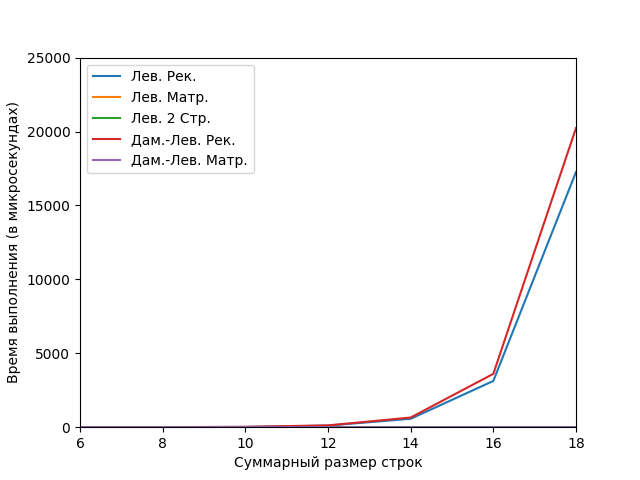
\includegraphics[scale = 0.85]{gr.png}
	\caption{Зависимость времени от суммарной длины строк}
	\label{fig:mpr6}
\end{figure}

\newpage

Время в микросекундах для всех реализаций представлено в таблице \ref{tb:times}.

\begin{table}[h!p]
	\begin{center}
		\caption{\label{tbl:time_test}Зависимость затрачиваемого процессорного времени от суммарной длины строк для алгоритмов}
		\label{tb:times}
		\begin{tabular}{|c|c|c|c|c|c|}
			\hline
			Суммарная длина строк & Лев. Рек. & Лев. Матр. & Лев. 2 Стр. & Дам.-Лев. Рек. & Дам.-Лев. Матр. \\ 
			\hline
            6 & 1.31 & 0.30 & 0.28 & 0.79 & 0.31 \\ 
            \hline
            8 & 3.79 & 0.41 & 0.38 & 4.34 & 0.47  \\ 
            \hline
            10 & 19.92 & 0.66 & 0.63 & 23.21 & 0.66  \\ 
            \hline
            12 & 106.72 & 0.82 & 0.81 & 122.97 & 1.02  \\ 
            \hline
            14 & 571.67 & 1.13 & 1.06 & 654.56 & 1.27  \\ 
            \hline
            16 & 3128.63 & 1.50 & 1.30 & 3609.66 & 1.76 \\ 
            \hline
            18 & 17262.44 & 1.73 & 1.59 & 20235.26 & 2.43 \\ 
            \hline
		\end{tabular}
	\end{center}
\end{table}

\section{Оценка затрачиваемой памяти}

Алгоритмы вычисления расстояний Левенштейна и Дамерау — Левенштейна не отличаются друг от друга с точки зрения использования памяти, следовательно, достаточно рассмотреть лишь разницу рекурсивной и матричной реализаций этих алгоритмов.

Максимальная глубина стека вызовов при рекурсивной реализации равна сумме длин входящих строк, соответственно, максимальный расход памяти вычисляется по формуле (\ref{for:99})
\begin{equation}
	(\mathcal{C}(S_1) + \mathcal{C}(S_2)) \cdot (2 \cdot \mathcal{C}\mathrm{(string)} + 2 \cdot \mathcal{C}\mathrm{(int)} + \mathcal{C}\mathrm{(bool)}),
	\label{for:99}
\end{equation}
где $\mathcal{C}$ — оператор вычисления размера, $S_1$, $S_2$ — строки, $\mathrm{int}$ — целочисленный тип, $\mathrm{string}$ — строковый тип,  $\mathrm{bool}$ - логический тип.

Использование памяти при итеративной реализации теоретически вычисляется по формуле (\ref{for:100}).
\begin{equation}
	(\mathcal{C}(S_1) + 1) \cdot (\mathcal{C}(S_2) + 1) \cdot \mathcal{C}\mathrm{(int)} + 5\cdot \mathcal{C}\mathrm{(int)} + 2 \cdot \mathcal{C}\mathrm{(string)})
	\label{for:100}
\end{equation}


\section*{Вывод}

Рекурсивный алгоритм вычисления расстояния Левенштейна работает на порядок дольше итеративных реализаций, время его работы увеличивается в геометрической прогрессии. На словах длиной 9 символов, матричная реализация алгоритма вычисления расстояния Левенштейна превосходит по времени работы рекурсивную почти в 10000 раз. Версия с двумя строками работает немного быстрее матричной реализации. 

Алгоритм вычисления расстояния Дамерау — Левенштейна используется для решения других задач, поэтому говорить о его отставании от алгоритма вычисления расстояния Левенштейна, исходя из временных затрат, некорректно.

По расходу памяти алгоритмы с использованием матрицы проигрывают рекурсивному: максимальный размер используемой памяти в них растёт как произведение длин строк, в то время как у рекурсивного алгоритма — как сумма длин строк.



\chapter*{Заключение}
\addcontentsline{toc}{chapter}{Заключение}

В рамках данной лабораторной работы были решены следующие задачи:

\begin{itemize}
	\item изучены и реализованны 5 алгоритмов расчета редакционного расстояния;
	\item протестированы реализованные алгоритмы;
	\item проведён сравнительный анализ алгоритмов по затраченному процессорному времени и памяти.
\end{itemize}

Поставленная цель, состоящая в получении навыка динамического программирования на примере реализации алгоритмов редакционного расстояния, достигнута.

\chapter*{Литература}
\addcontentsline{toc}{chapter}{Литература}
\begin{enumerate}
	\item Свойство Process.UserProcessorTime [Электронный ресурс]. Режим доступа: https://docs.microsoft.com/ru-ru/dotnet/api/system.diagnostics.stopwatch?view=net-5.0. Дата обращения: 01.10.2021
\end{enumerate}


\end{document}
